\chapter{Experiments}
\label{sec:experiments}

This chapter will cover the experiments implemented throughout this project, which focused on reducing data sets with the presented algorithms and evaluating these reductions. Once again, it is quite difficult to evaluate reductions, but a set of metrics were adopted to attempt to understand them as much as possible.

First, let $\vect X_{n \times f}$ be a data set with $n$ samples and $f$ features, and $\vect D \subset \mathbb{N} \mid d \in \vect D \implies d \le f$ a  set of dimensions to which $\vect X$ should be reduced. Additionally, consider the score to be the class prediction accuracy or the coefficient of determination $R^2$, depending on the nature (classification or regression) of the problem of interest. Then, the sequence bellow represents a default format followed by all experiments:

\begin{enumerate}
	\item The data set $\vect X$ is loaded and its first three features are plotted, given an initial idea of how the data is distributed for those features.
	\item $\vect X$ is reduced to 3, 2 and 1 dimensions. Each reduction is plotted for visualization.
	\item Kruskal's stress is calculated for $\vect X$.
	\item In an attempt to evaluate local dissimilarity preservation, a 1-NN classifier or regressor is trained with 80\% of $\vect X$'s samples and tested with the other 20\%. The score is kept for future reference.
	\item Grid search is executed over $\vect X$ using a SVM classifier or regressor. This step evaluates how a ``real world" algorithm would perform over the original data set.
	\item for $d \in \vect D$:
	\begin{enumerate}
		\item $\vect X$ is embedded into the $\mathbb{R}^d$, creating the data set $\vect Y_{n \times d}$.
		\item Kruskal's stress is calculated for $\vect Y$.
		\item A 1-NN classifier or regressor is trained with the same samples used in step 4, and tested with all the others. The score is compared to the one retrieved in step 4.
		\item Grid Search is executed over $\vect Y$ and the score is compared to the one presented in step 5.
	\end{enumerate}
\end{enumerate}

\section{K Data Set}

The synthetic data set $\vect K$, with 1000 samples and 2 features.

\begin{figure}[H]
	\centering
	\captionsetup{justification=centering}
	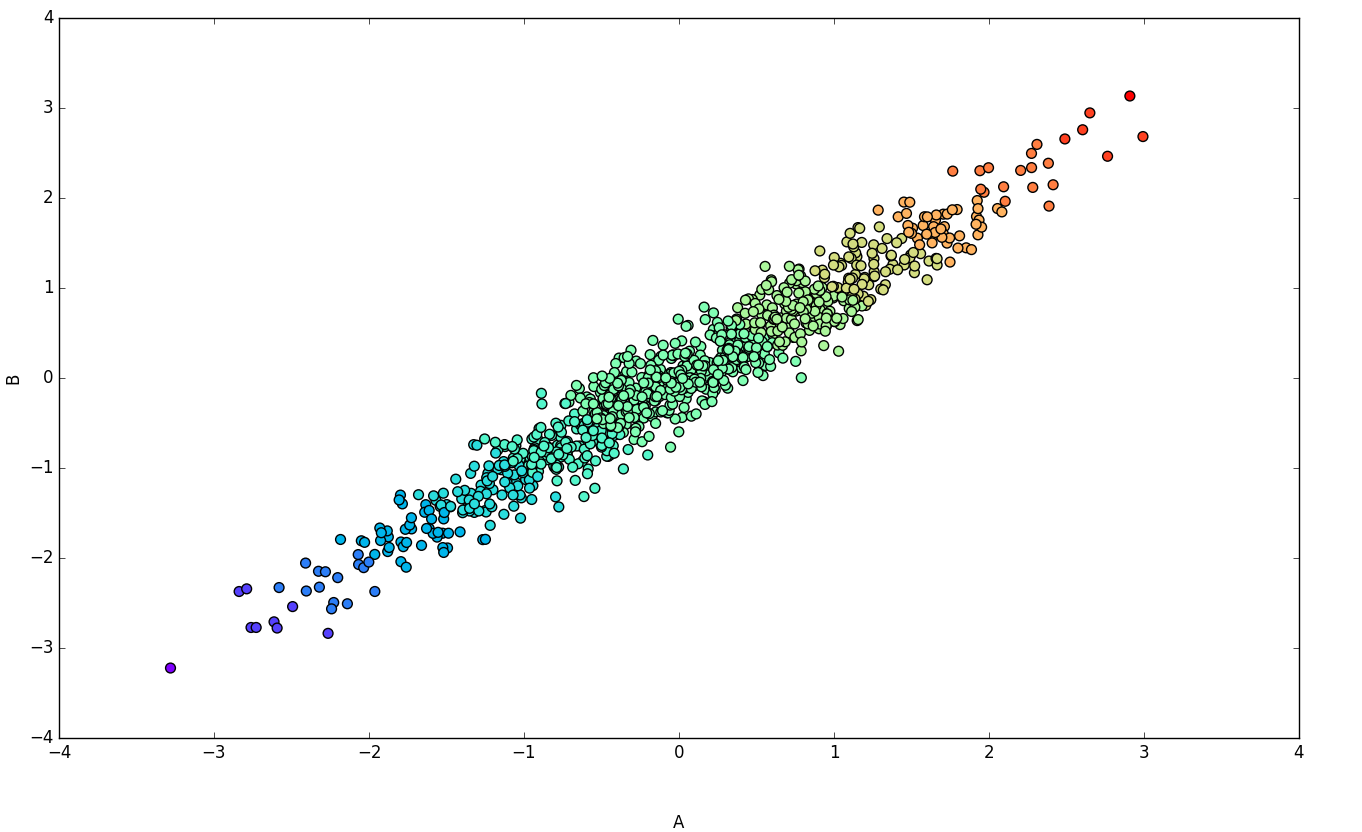
\includegraphics[width=\linewidth]{datasets/r}
	\caption{The $\vect K$ data set.}
\end{figure}

\begin{figure}[H]
	\centering
	\captionsetup{justification=centering}
	
	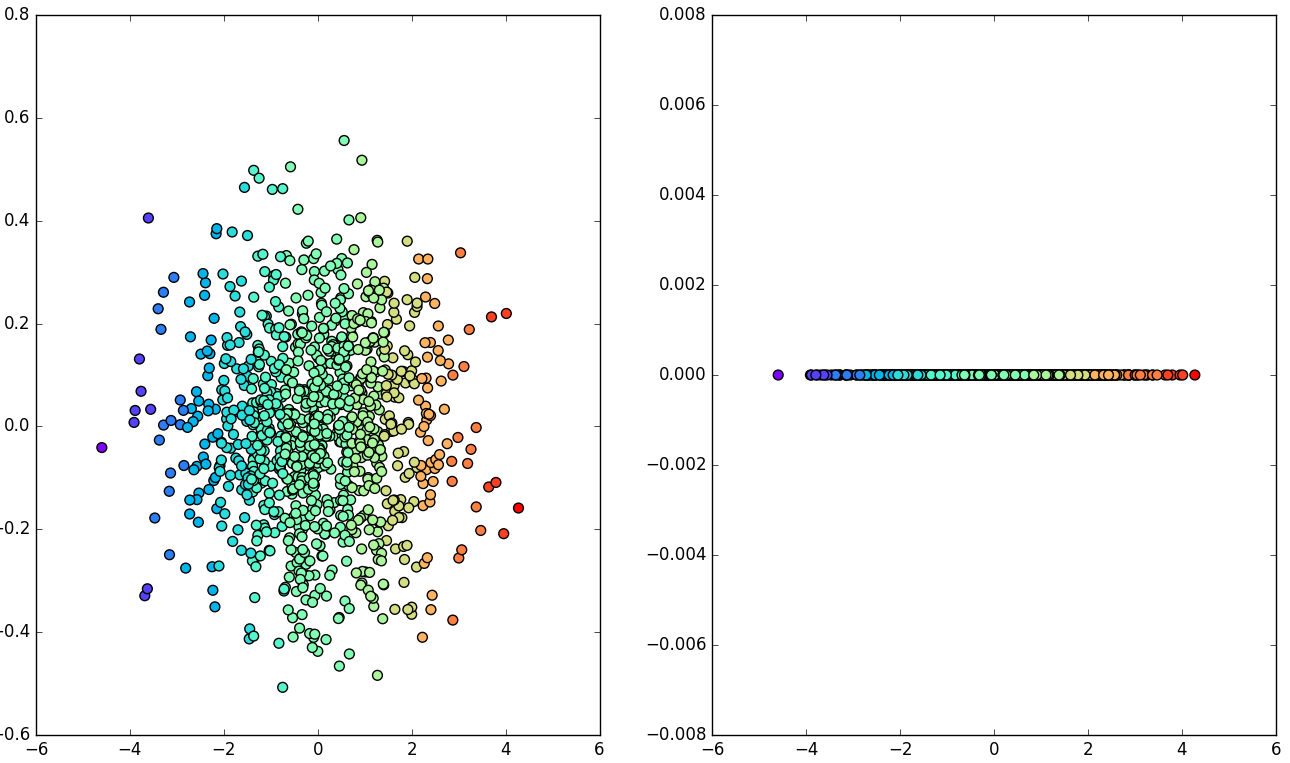
\includegraphics[width=\linewidth]{experiments/pca_k}
	\caption{The reductions of $\vect K$ to 2 and 1 dimension, respectively.}
	\label{fig:dsrpca}
\end{figure}

Figure \ref{fig:dsrpca} illustrates the results of PCA algorithm application over $\vect K$ data set. Notice that, for the second application, it correctly chose to discard the vertical dimension, as the samples offer less variability in this component.

\begin{table}[H]
	\centering
	\begin{tabular}{|p{.25\linewidth}|p{.20\linewidth}|p{.20\linewidth}|p{.20\linewidth}|}
		\hline
		& \textbf{Original $\mathbb{R}^2$} & \textbf{$\mathbb{R}^2$} & \textbf{$\mathbb{R}$} \\\hline
		\textbf{1-NN} & .99 & .99 & 1 \\\hline
		\textbf{Score} & .982 & .982 & .994 \\\hline
		\textbf{Best parameters} & 'C': 1000, 'k': 'linear' & 'C': 1000, 'k': 'linear' & 'C': 1000, 'g': 10, 'k': rbf \\\hline
		\textbf{GridSearch time} & 2.55 s s & 2.93 s & 2.94 s \\\hline
		\textbf{Reduction time} & - & 1.97 s & 1.93 s \\\hline
		\textbf{Kruskal's stress} & - & 0 & .0399 \\\hline
		\textbf{Data size} & 15.62 KB & 15.62 KB & 7.81 KB \\\hline
	\end{tabular}
	\captionsetup{justification=centering}
	\caption{Description of predictions and reduction performance for $\vect K$.}
\end{table}

From the table above, one can see that, given the linear nature of $\vect K$, PCA was an adequate method to reduce it, as both 1-NN regressor and SVM created very accurate models. It is also possible to observe how Kruskal's stress might not be an appropriate quality measurement, given a specific domain. Indeed, $\vect K$'s stress increase resulted from the removal of one of the components did not imply on prediction accuracy decrease.

\clearpage
\section{The Iris Flower Data Set}

The Iris Flower data set, as presented in section \ref{irisdataset}, containing 150 samples and 4 features.

\begin{figure}[H]
	\centering
	\captionsetup{justification=centering}
	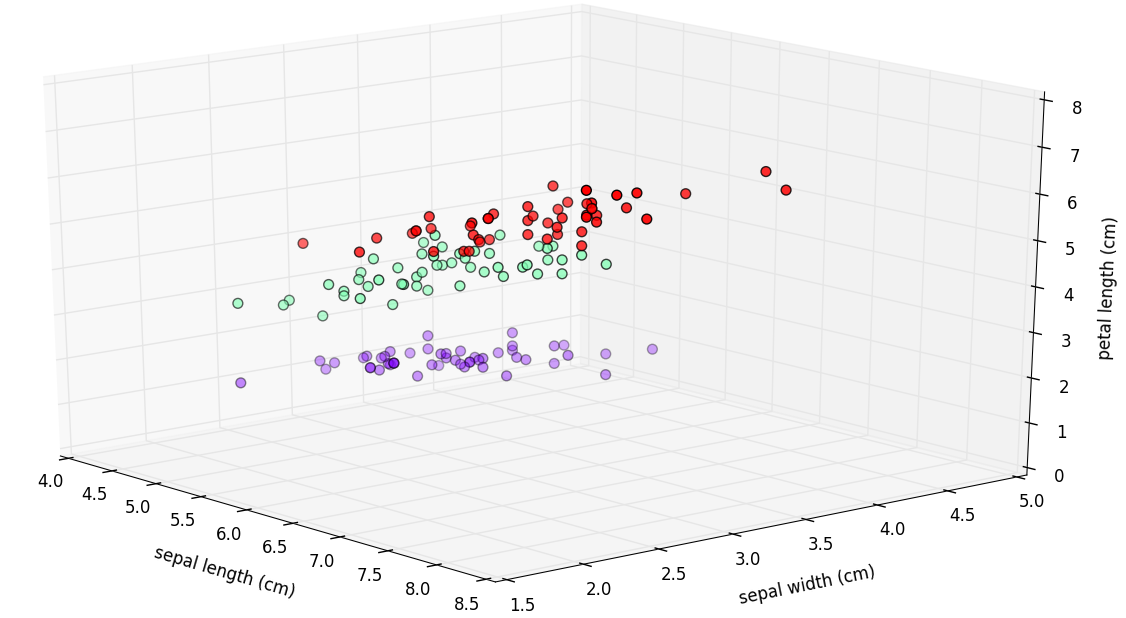
\includegraphics[width=\linewidth]{datasets/iris}
	\caption{The Iris Flower data set.}
\end{figure}

\newpage
\paragraph{Reducing the Iris Flower Data Set With the PCA Algorithm}

\begin{figure}[H]
	\centering
	\captionsetup{justification=centering}
	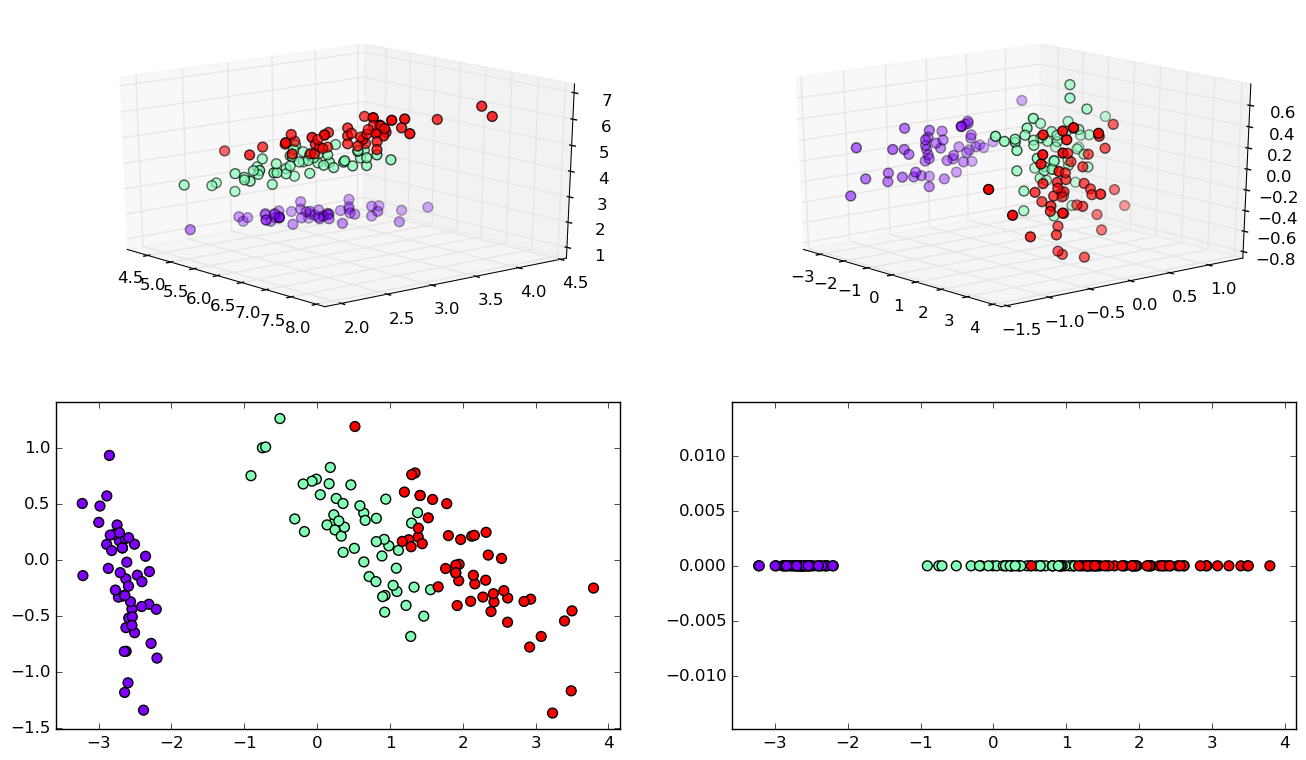
\includegraphics[width=\linewidth]{experiments/pca_iris}
	\caption{The reductions of Iris Flower to 3, 2, and 1 dimensions, respectively, using the PCA algorithm.}
	\label{fig:dsirispca}
\end{figure}

One can infer from figure \ref{fig:dsirispca} that classes are still somewhat organized in different clusters, even in the reductions for 2 and 1 dimensions. The Application of PCA therefore results in fairly good visualizations.

\begin{table}[H]
	\centering
	
	\begin{tabular}{|p{.25\linewidth}|p{.15\linewidth}|p{.15\linewidth}|p{.15\linewidth}|p{.15\linewidth}|}
		\hline
		& \textbf{Original} & $\mathbb{R}^3$ & $\mathbb{R}^2$ & $\mathbb{R}$ \\\hline
		\textbf{1-NN} & 1 & 1 & 1 & .87 \\\hline
		\textbf{Score} & .99 & .98 & .97 & .95 \\\hline
		\textbf{Best parameters} & g: .01, k: rbf, C: 100 & k: linear, C: 10 & g: 10, k: rbf, C: 1 & g: .1, k: sigmoid, C: 1 \\\hline
		\textbf{GridSearch time} & 2.14 s & 2.64 s & 2.42 s & 2.64 s \\\hline
		\textbf{Reduction time} & - & .17 s & .17 s & .16 s \\\hline
		\textbf{Kruskal's stress} & - & .01 & .04 & .11 \\\hline
		\textbf{Data size} & 4.69 KB & 3.52 KB & 2.34 KB & 1.17 KB \\\hline
	\end{tabular}
	
	\captionsetup{justification=centering}
	\caption{Description of predictions and reduction performance for the Iris flower and PCA algorithm.}
\end{table}

Kruskal's stress kept bellow 11\% for all reductions. Indeed, variations in the learning phase performance were small: 1-NN and SVM score were high along all reductions (except for the last one, perhaps, where 1-NN decreased to .87).

\paragraph{Reducing the Iris Flower Data Set With the ISOMAP Algorithm}

\begin{figure}[H]
	\centering
	\captionsetup{justification=centering}
	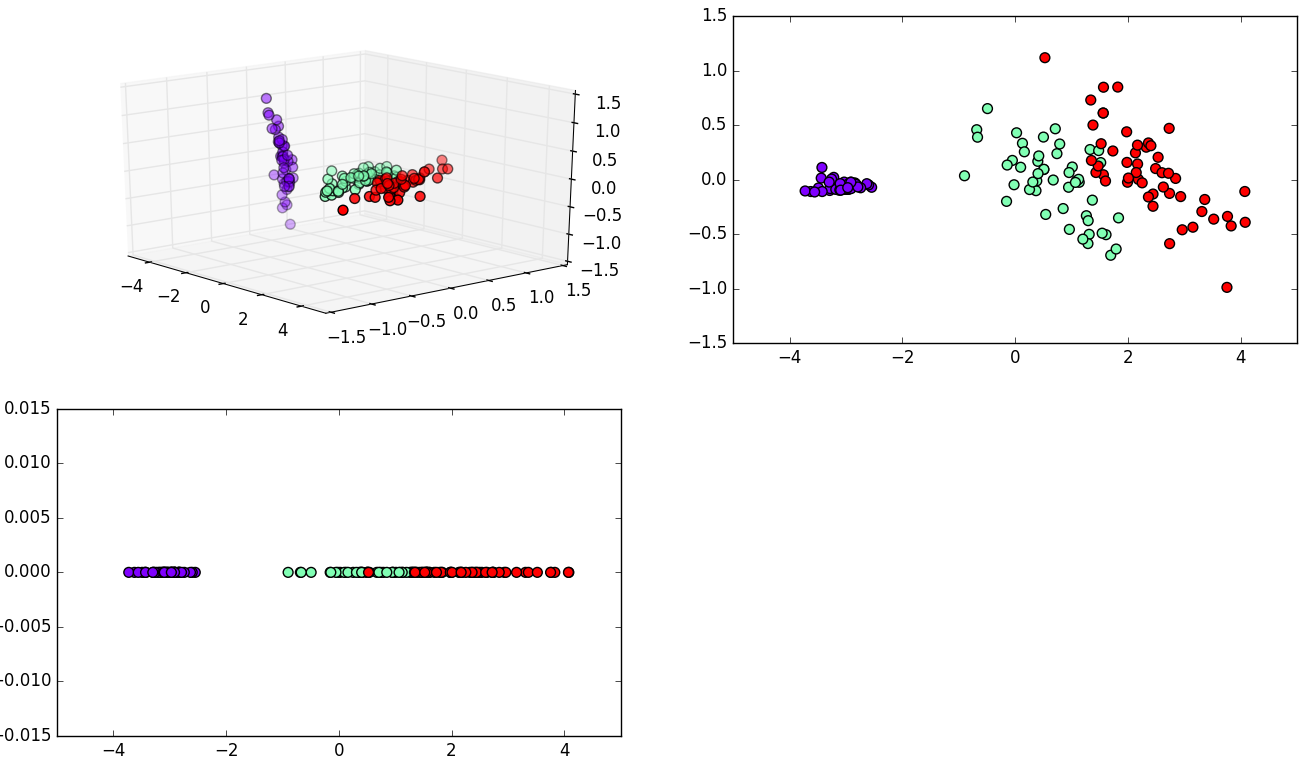
\includegraphics[width=\linewidth]{experiments/iso_iris}
	\caption{The reductions of Iris Flower to 3, 2, and 1 dimensions, respectively, using the ISOMAP algorithm.}
	\label{fig:dsirisiso}
\end{figure}

It is clear, from figure \ref{fig:dsirisiso}, that the ISOMAP algorithm has also resulted in acceptable reductions of the Iris Flower data set, where classes kept a similar organization compared to the reductions made by the PCA algorithm.

\begin{table}[H]
	\centering
	
	\begin{tabular}{|p{.25\linewidth}|p{.15\linewidth}|p{.15\linewidth}|p{.15\linewidth}|p{.15\linewidth}|}
		\hline
		& \textbf{Original} & $\mathbb{R}^3$ & $\mathbb{R}^2$ & $\mathbb{R}$ \\\hline
		\textbf{1-NN} & 1 & 1 & 1 & .87 \\\hline
		\textbf{Pred. accuracy} & .99 & .98 & .98 & .93 \\\hline
		\textbf{Best parameters} & k: rbf, g: 0.01, C: 100 & k: linear, C: 10 & k: linear, C: 10 & k: sigmoid, g: 0.1, C: 1 \\\hline
		\textbf{GridSearch time} & 2 s & 2.55 s & 2.42 s & 2.37 s \\\hline
		\textbf{Reduction time} & - & 1.28 s & 1.3 s & 1.27 s \\\hline
		\textbf{Kruskal's stress} & - & .15 & .15 & .16 \\\hline
		\textbf{Data size} & 4.69 KB & 3.52 KB & 2.34 KB & 1.17 KB \\\hline
	\end{tabular}
	\captionsetup{justification=centering}
	\caption{Description of predictions and reduction performance for the Iris flower and ISOMAP algorithm.}
\end{table}

The results were very similar to the ones obtained when applying the PCA algorithm. The disparities consist on the Kruskal's stress, which is now limited to 16\% and the reduction time, which has consistently increased considering the higher computational cost of the ISOMAP algorithm.

\clearpage
\section{The Digits Data Set}

Digits data set is composed by 1797 samples, 64 features and 10 classes. Each sample is a 8x8 image of a hand-written digit from 0 to 9.

\begin{figure}[H]
	\centering
	\captionsetup{justification=centering}
	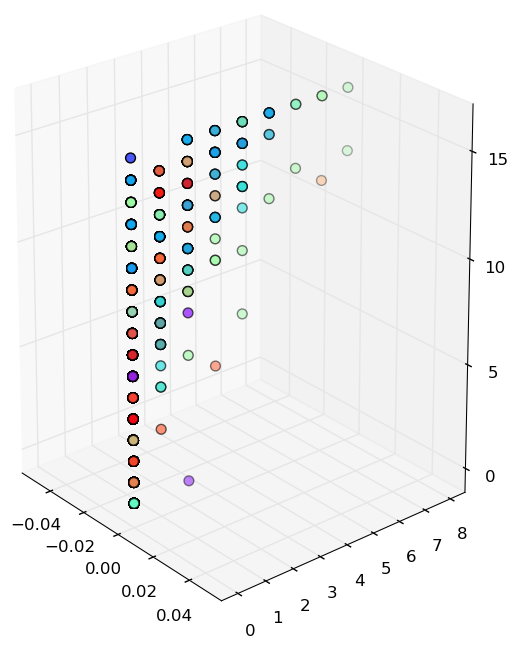
\includegraphics[width=\linewidth]{datasets/digits}
	\caption{The Digits data set.}
\end{figure}

\newpage
\paragraph{Reducing the Digits Data Set With the PCA Algorithm}

\begin{figure}[H]
	\centering
	\captionsetup{justification=centering}
	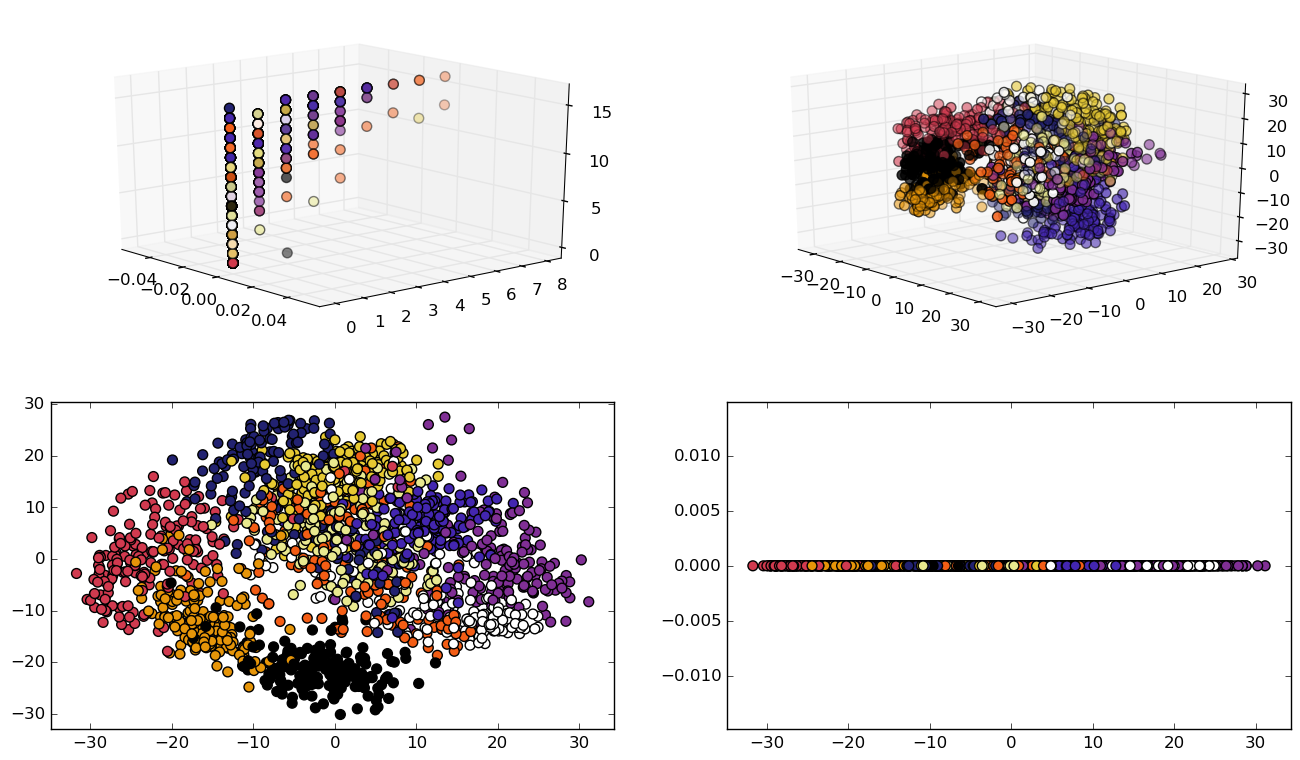
\includegraphics[width=\linewidth]{experiments/pca_digits}
	\caption{The reductions of Digits to 3, 2 and 1 dimensions, respectively, with the PCA algorithm.}
	\label{fig:dsdigitspca}
\end{figure}

From figure \ref{fig:dsdigitspca}, we have glimpse of Digits's samples structure. The many classes' clusters are visible in the 3D, although they become highly mixed in the 2D and 1D, yielding a confusing representation.

\begin{table}[H]
	\centering
	
	\begin{tabular}{|p{.14\linewidth}|p{.14\linewidth}|p{.14\linewidth}|p{.14\linewidth}|p{.14\linewidth}|p{.14\linewidth}|}
		\hline
		& \textbf{Original} & $\mathbb{R}^{10}$ & $\mathbb{R}^3$ & $\mathbb{R}^2$ & $\mathbb{R}$ \\\hline
		\textbf{1-NN} & .99 & .97 & .68 & .56 & .28 \\\hline
		\textbf{Score} & .98 & .95 & .74 & .64 & .39  \\\hline
		\textbf{Best parameters} & k: rbf, C: 10, g: .001 & k: rbf, C: 10, g: .001 & k: rbf, C: 10, g: .01 & k: rbf, C: 1, g: .01 & k: rbf, C: 10, g: .001\\\hline
		\textbf{GridSearch time} & 11.75 s & 26.97 s & 150.91 s & 125.64 s & 104.41 s \\\hline
		\textbf{Reduction time} & - & 6.02 s & 6.54 s & 6.05 s & 6.1 s \\\hline
		\textbf{Kruskal's stress} & - & .16 & .42 & .54 & .71 \\\hline
		\textbf{Data size} & 898.5 KB & 140.4 KB & 42.1 KB & 28.08 KB & 14 KB \\\hline
	\end{tabular}
	
	\caption{Description of predictions and reduction performance for Digits and ISOMAP algorithm.}
\end{table}

Notice that it was possible to eliminate 54 dimensions, consistently reducing the data set size, and only suffering 3\% of prediction accuracy loss. The score drastically decreased, however, when more dimensions were removed. Furthermore, reductions to less than 10 dimensions would generate highly mixed samples, requiring more time for grid searching. Finally, it is also clear that score was inversely proportional to stress.

\paragraph{Reducing the Digits Data Set With the ISOMAP Algorithm}

\begin{figure}[H]
	\centering
	\captionsetup{justification=centering}
	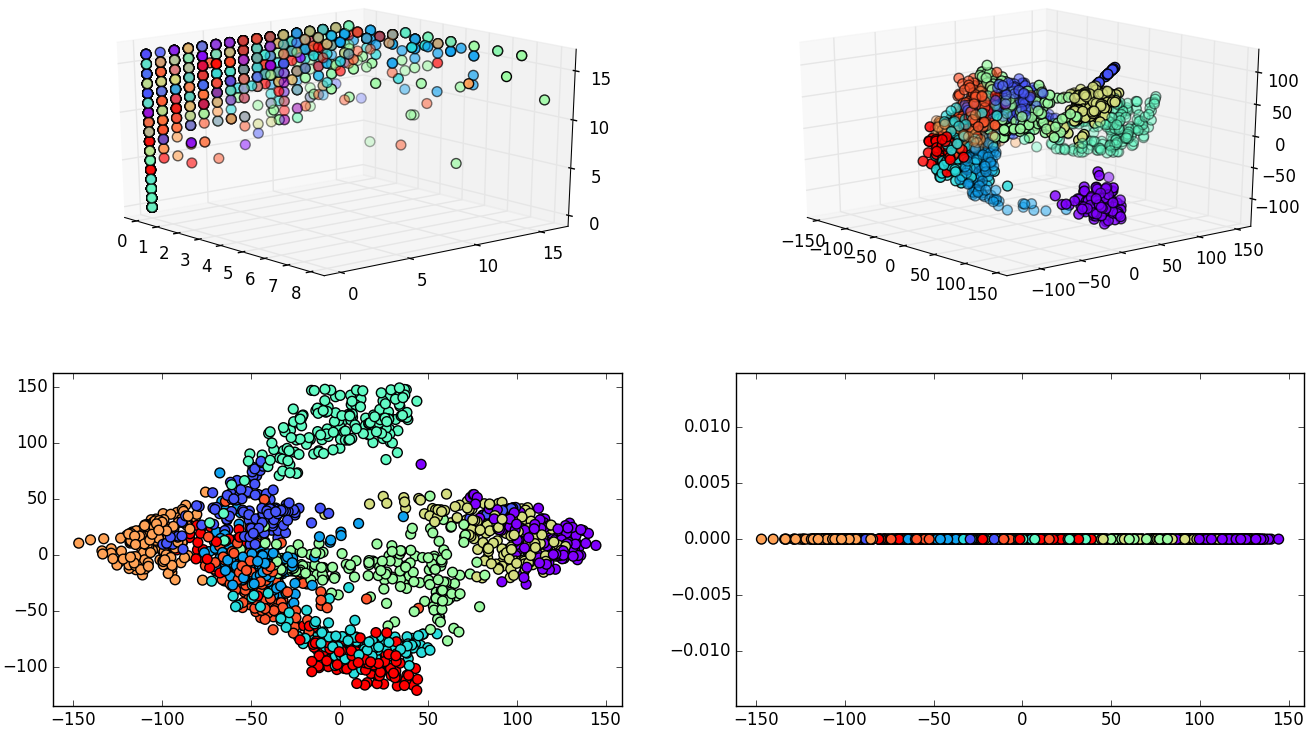
\includegraphics[width=\linewidth]{experiments/iso_digits}
	\caption{The reductions of Digits to 3, 2 and 1 dimensions, respectively, with the ISOMAP algorithm.}
	\label{fig:dsdigitsiso}
\end{figure}

Digits reductions using ISOMAP, as illustrated in figure \ref{fig:dsdigitsiso}, have proven to be much more organized, when compared to the reductions made by the PCA algorithm. Indeed, the representation in the 2D shows much less mixed samples, which translates into better scores:

\begin{table}[H]
	\centering
	
	\begin{tabular}{|p{.14\linewidth}|p{.14\linewidth}|p{.14\linewidth}|p{.14\linewidth}|p{.14\linewidth}|p{.14\linewidth}|}
		\hline
		& \textbf{Original} & $\mathbb{R}^{10}$ & $\mathbb{R}^3$ & $\mathbb{R}^2$ & $\mathbb{R}$ \\\hline
		\textbf{1-NN} & .99 & .99 & .97 & .92 & .46 \\\hline
		\textbf{Score} & & & & & \\\hline
		\textbf{Best parameters} & & & & & \\\hline
		\textbf{GridSearch time} & 7.68 s & 5.1 s & 4.59 s & 4.47 s & 5.44 s \\\hline
		\textbf{Reduction time} & - & 47.93 s & 47.99 s & 48.31 s & 48.82 s \\\hline
		\textbf{Kruskal's stress} & - & .16 & .42 & .54 & .71 \\\hline
		\textbf{Data size} & 898.5 KB & 140.4 KB & 42.1 KB & 28.08 KB & 14 KB \\\hline
	\end{tabular}
	
	\caption{Description of predictions and reduction performance for Digits and ISOMAP algorithm.}
\end{table}

\clearpage
\section{The Swiss Roll Data Set}

The Swiss Roll data set, with 1000 samples and 3 features.

\begin{figure}[H]
	\centering
	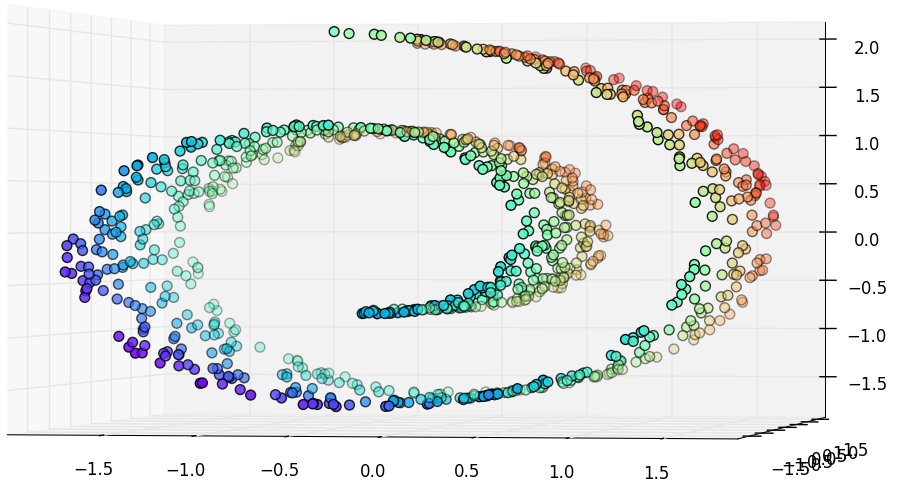
\includegraphics[width=\linewidth]{datasets/swiss}
	\captionsetup{justification=centering}
	\caption{The Swiss Roll data set.}
\end{figure}

\newpage
\paragraph{Reducing the Swiss Roll Data Set With the PCA Algorithm}

\begin{figure}[H]
	\centering
	\captionsetup{justification=centering}
	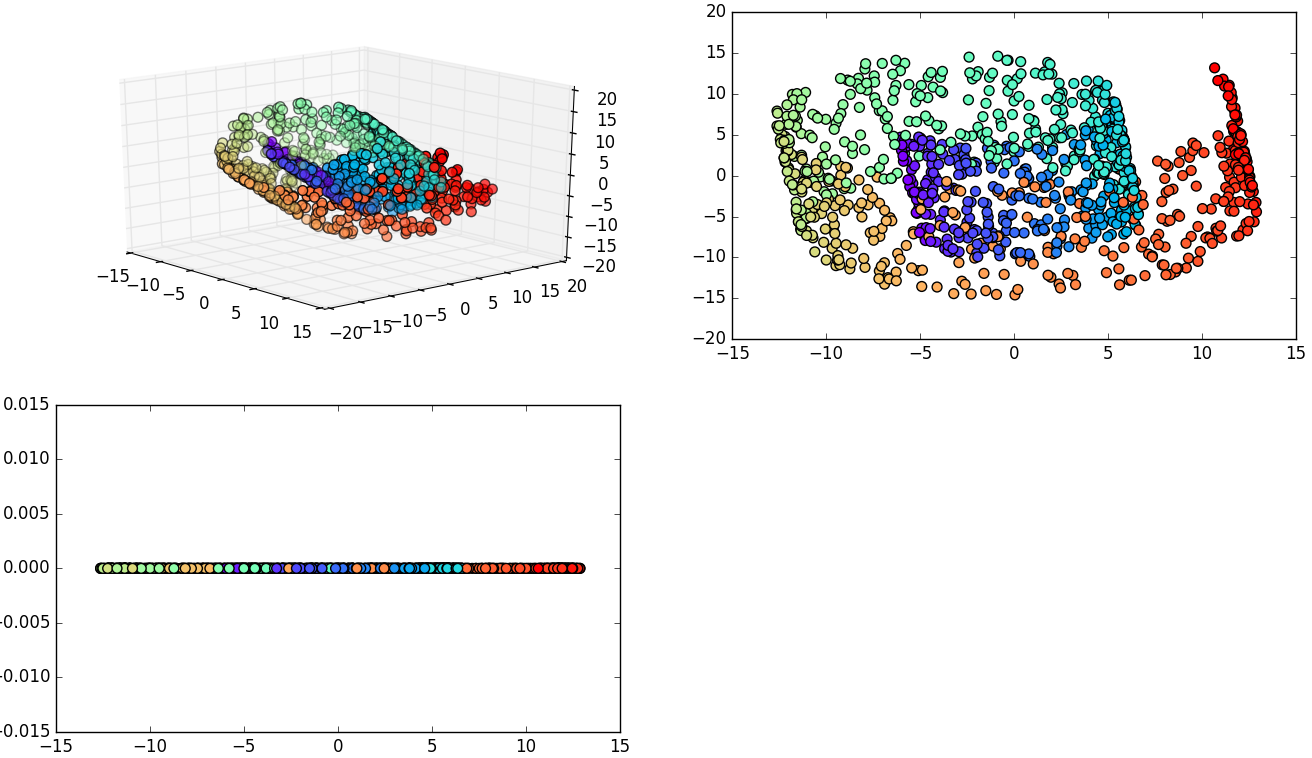
\includegraphics[width=\linewidth]{experiments/pca_swiss}
	\caption{The reductions of the Swiss Roll to 3, 2 and 1 dimensions, respectively, with the PCA algorithm.}
	\label{fig:dsswisspca}
\end{figure}

Figure \ref{fig:dsswisspca} illustrates how the PCA algorithm is not suitable for reducing the Swiss-roll, given its non-linear distribution. Reductions to 2 and 1 dimensions have made very dissimilar samples to become mixed, damaging the original structure of the data set and, of course, decreasing score in the learning process:

...

\paragraph{Reducing the Swiss Roll Data Set With the ISOMAP Algorithm}

\begin{figure}[H]
	\centering
	\captionsetup{justification=centering}
	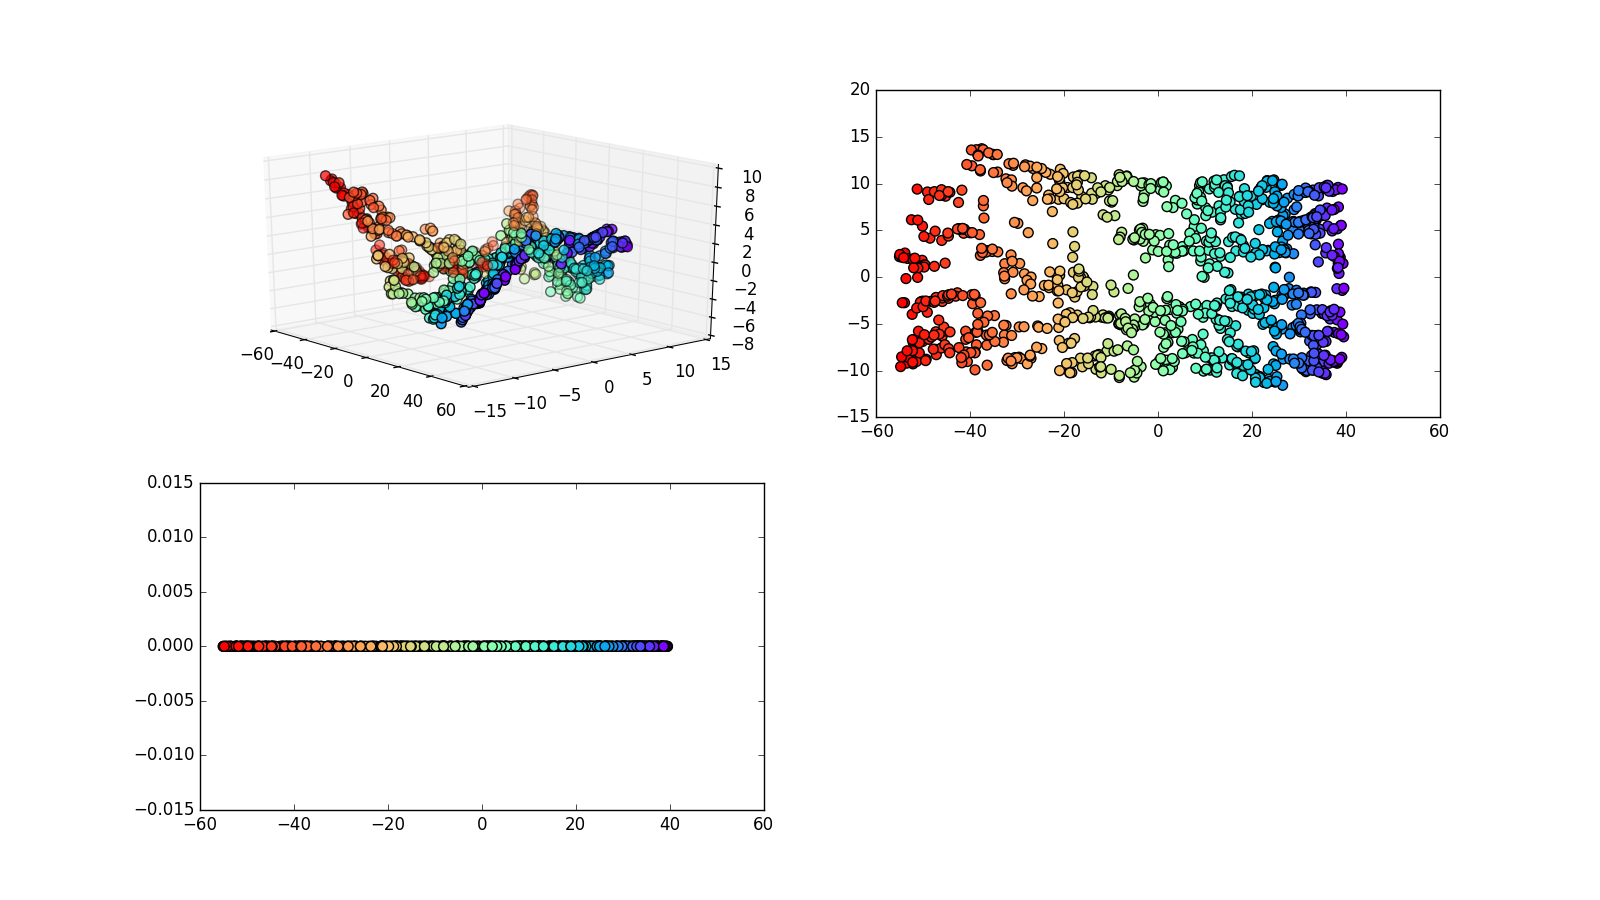
\includegraphics[width=\linewidth]{experiments/iso_swiss}
	\caption{The reductions of the Swiss Roll to 3, 2 and 1 dimensions, respectively, with the ISOMAP algorithm.}
	\label{fig:dsswissiso}
\end{figure}

Figure \ref{fig:dsswissiso} illustrates the efficacy of the ISOMAP algorithm in reducing the Swiss Roll while still preserving the original structure of the data set (similar samples were maintained close to each other). This has, of course, a positive impact on learning:

...

\clearpage
\section{The Glass Data Set}

The Glass data set contains 214 samples and 10 features, were the first one is the identification number of a given sample.

\begin{figure}[H]
	\centering
	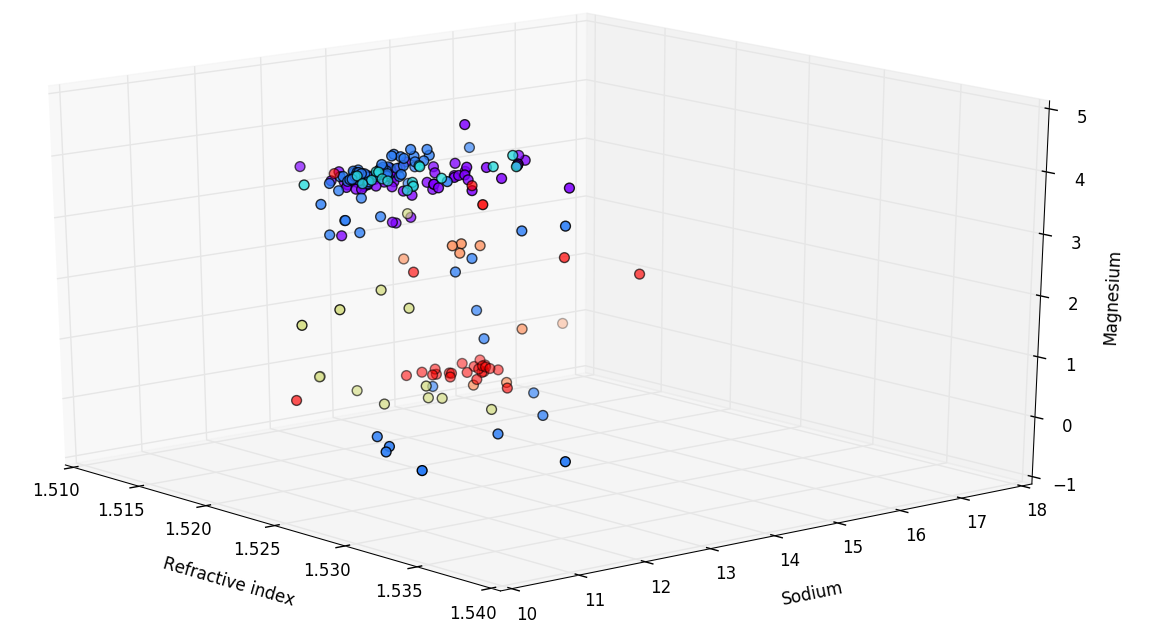
\includegraphics[width=\linewidth]{datasets/glass}
	\captionsetup{justification=centering}
	\caption{The Glass data set.}
\end{figure}

\newpage
\paragraph{Reducing the Glass Data Set With the ISOMAP Algorithm}

\begin{figure}[H]
	\centering
	\captionsetup{justification=centering}
	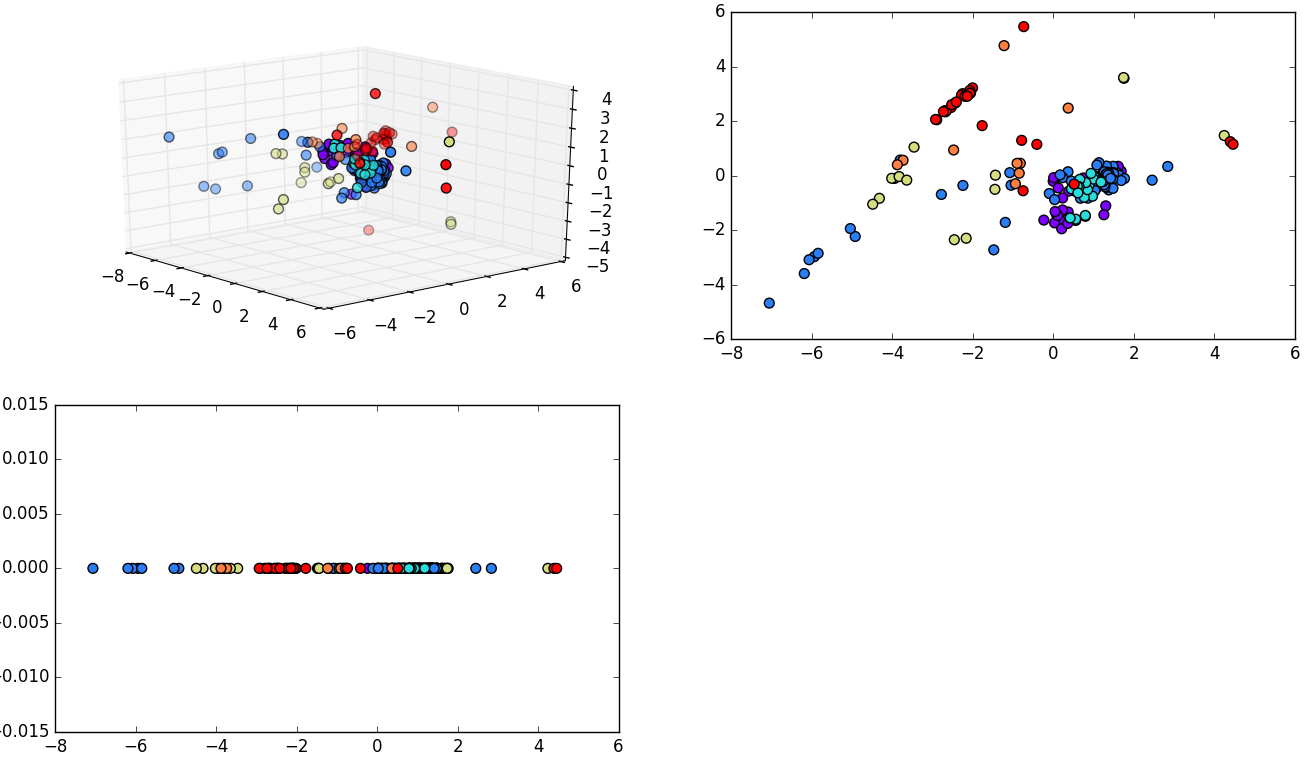
\includegraphics[width=\linewidth]{experiments/iso_glass}
	\caption{The reductions of Glass to 3, 2 and 1 dimensions, respectively, with the ISOMAP algorithm.}
	\label{fig:dsglassiso}
\end{figure}

\clearpage
\section{The Dermatology Data Set}

The Dermatology data set, composed by 366 samples and 35 features. Here, the target is to correctly diagnose the erythemato-squamous diseases.

\begin{figure}[H]
	\centering
	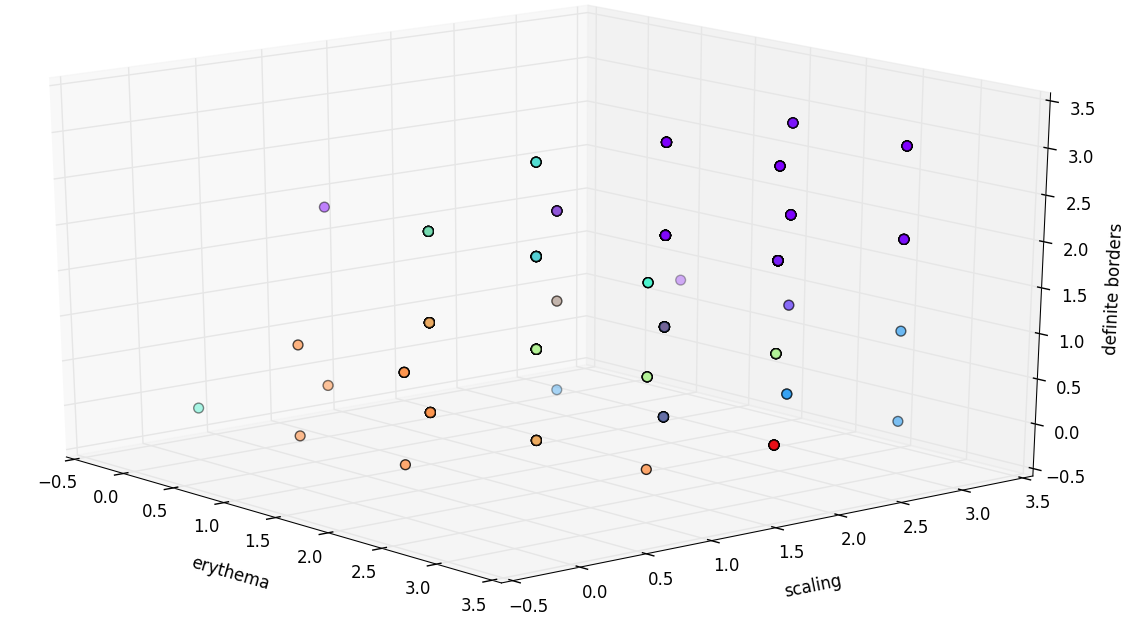
\includegraphics[width=\linewidth]{datasets/dermatology}
	\captionsetup{justification=centering}
	\caption{The Dermatology data set.}
\end{figure}

\newpage
\paragraph{Reducing the Dermatology Data Set With the ISOMAP Algorithm}

\begin{figure}[H]
	\centering
	\captionsetup{justification=centering}
	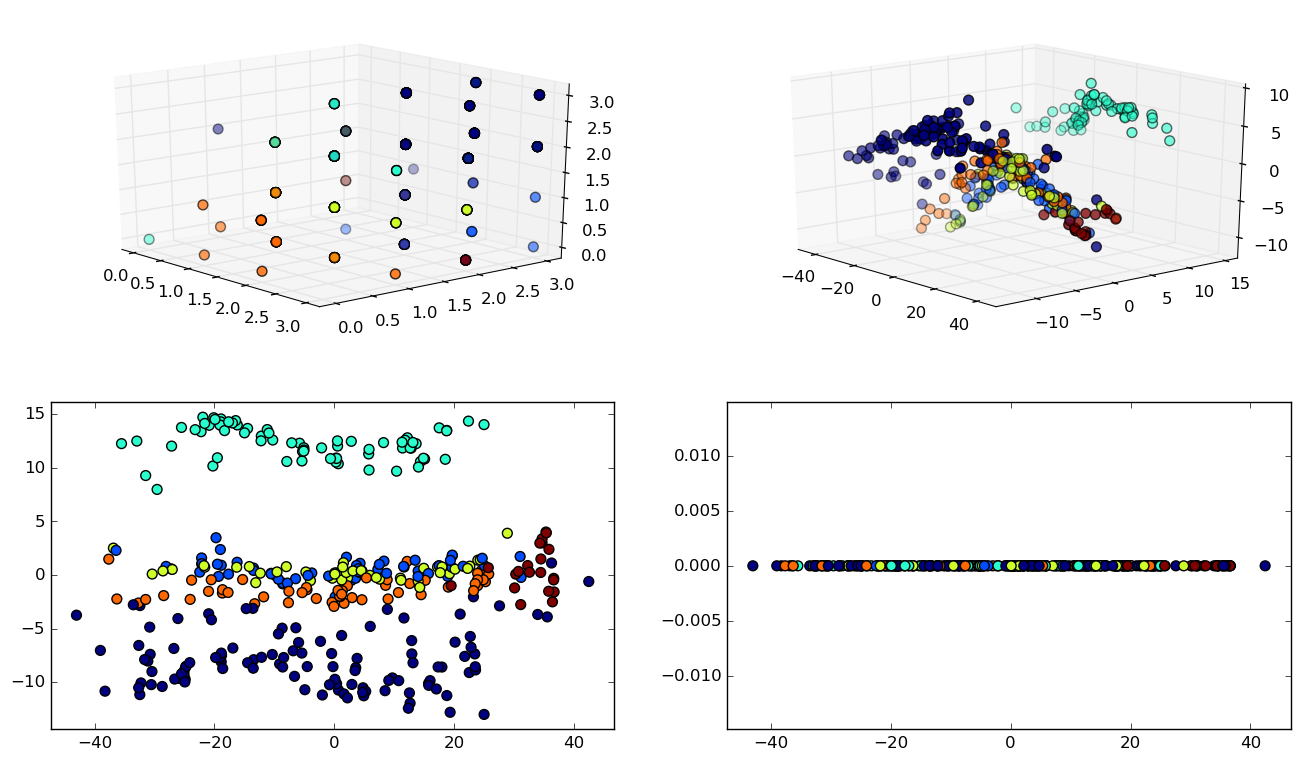
\includegraphics[width=\linewidth]{experiments/iso_dermatology}
	\caption{The reductions of Dermatology to 3, 2 and 1 dimensions, respectively, with the ISOMAP algorithm.}
	\label{fig:dsdermatologyiso}
\end{figure}

\clearpage
\section{The Leukemia Data Set}

The Leukemia data set contains 72 samples and 7129 features, which express levels of the genes in a given patient. Each sample belongs to a class $t \in \{-1, 1\}$, tagging which of two variants of leukemia is present in the sample (AML, 25 samples, or ALL, 47 samples) \cite{on:duc_ds}.

\begin{figure}[H]
	\centering
	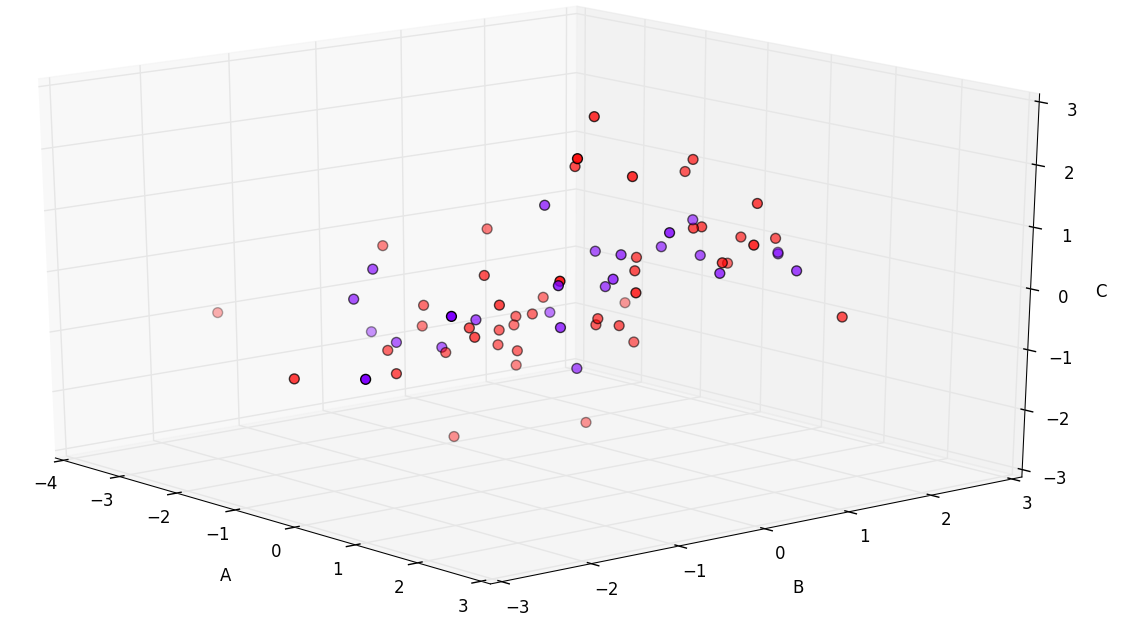
\includegraphics[width=\linewidth]{img/datasets/leukemia}
	\captionsetup{justification=centering}
	\caption{The Leukemia data set.}
\end{figure}

\newpage
\paragraph{Reducing the Dermatology Data Set With the ISOMAP Algorithm}

\begin{figure}[H]
	\centering
	\captionsetup{justification=centering}
	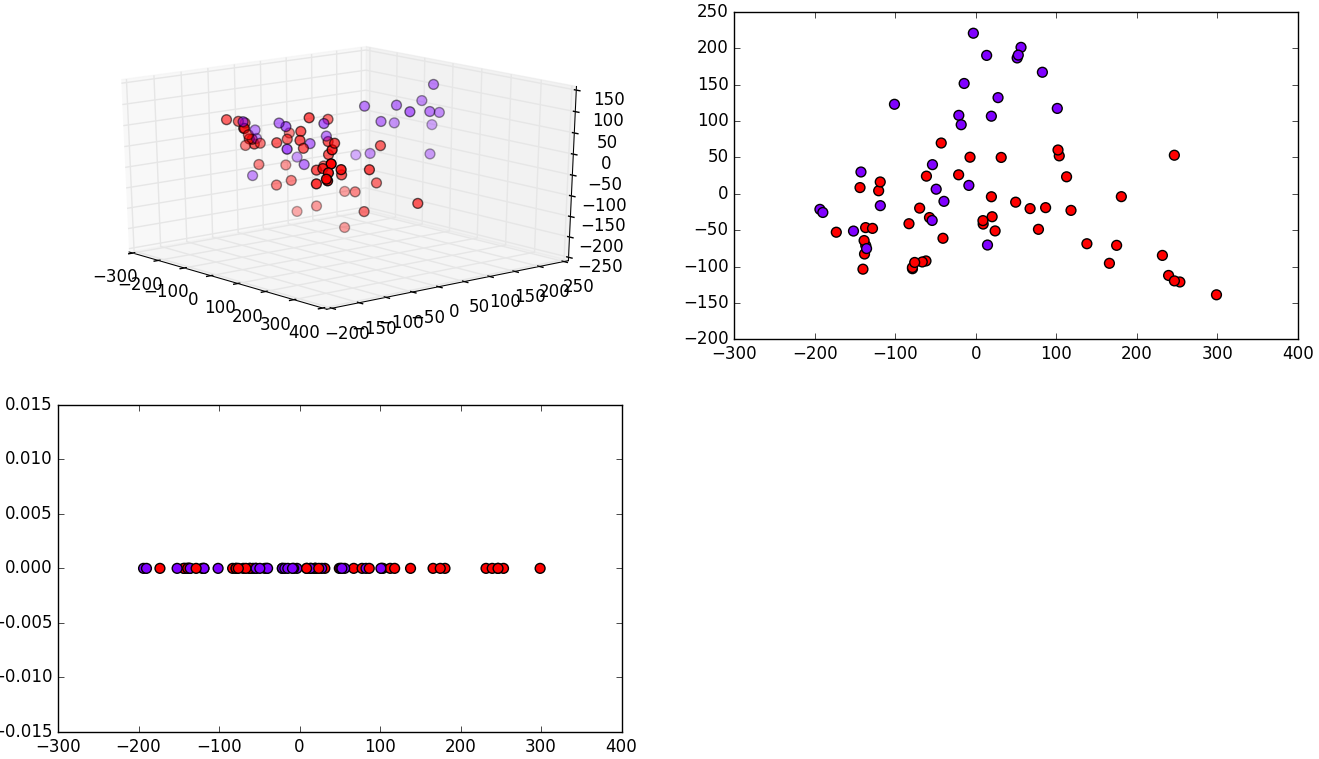
\includegraphics[width=\linewidth]{experiments/iso_leukemia}
	\caption{The reductions of Leukemia to 3, 2 and 1 dimensions, respectively, with the ISOMAP algorithm.}
	\label{fig:dsleukemiaiso}
\end{figure}

The Results in this experiment are quite impressive: although visualization has barely changed from 7129 to 3 dimensions, a 7129-dimensional space was reduced to a 10-dimensional one with only 10\% of accuracy loss.

\clearpage
\subsection{The WDBC Data Set}

The Wisconsin Diagnostic Breast Cancer (WDBC) data set, containing 596 samples and 32 features computed from a breast mass. WDBC has 357 benign samples and 212 malignant. During this experiment, the first feature was disregarded, as it represents the identification numbers of the samples.

\begin{figure}[H]
	\centering
	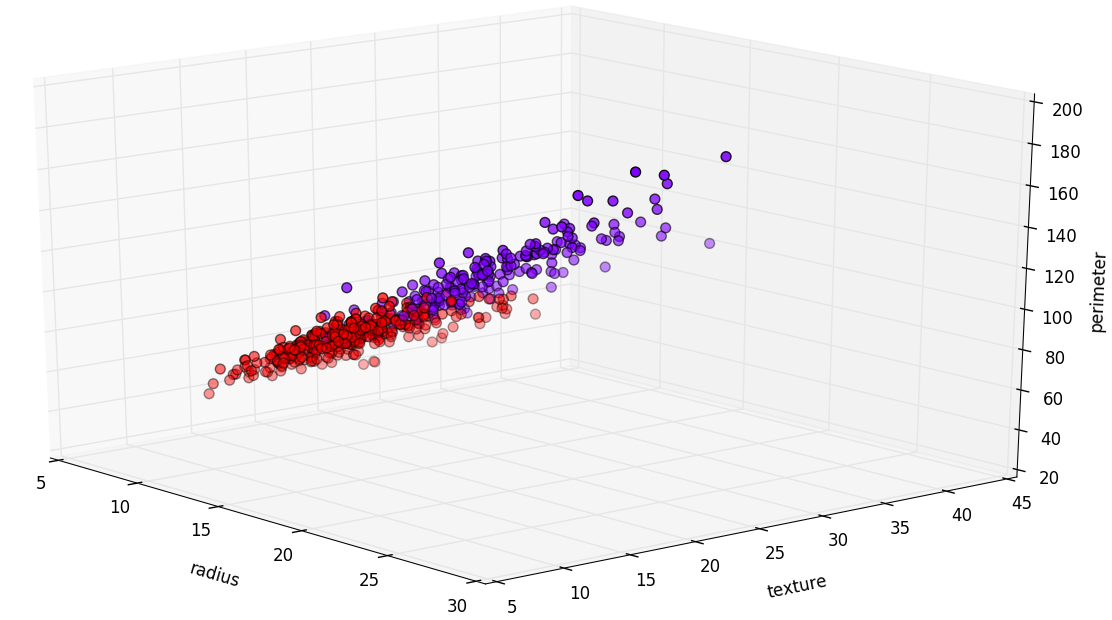
\includegraphics[width=\linewidth]{img/datasets/wdbc}
	\captionsetup{justification=centering}
	\caption{The WDBC data set.}
	\label{fig:dswdbc}
\end{figure}

\newpage
\paragraph{Reducing the WDBC Data Set With the ISOMAP Algorithm}

\begin{figure}[H]
	\centering
	\captionsetup{justification=centering}
	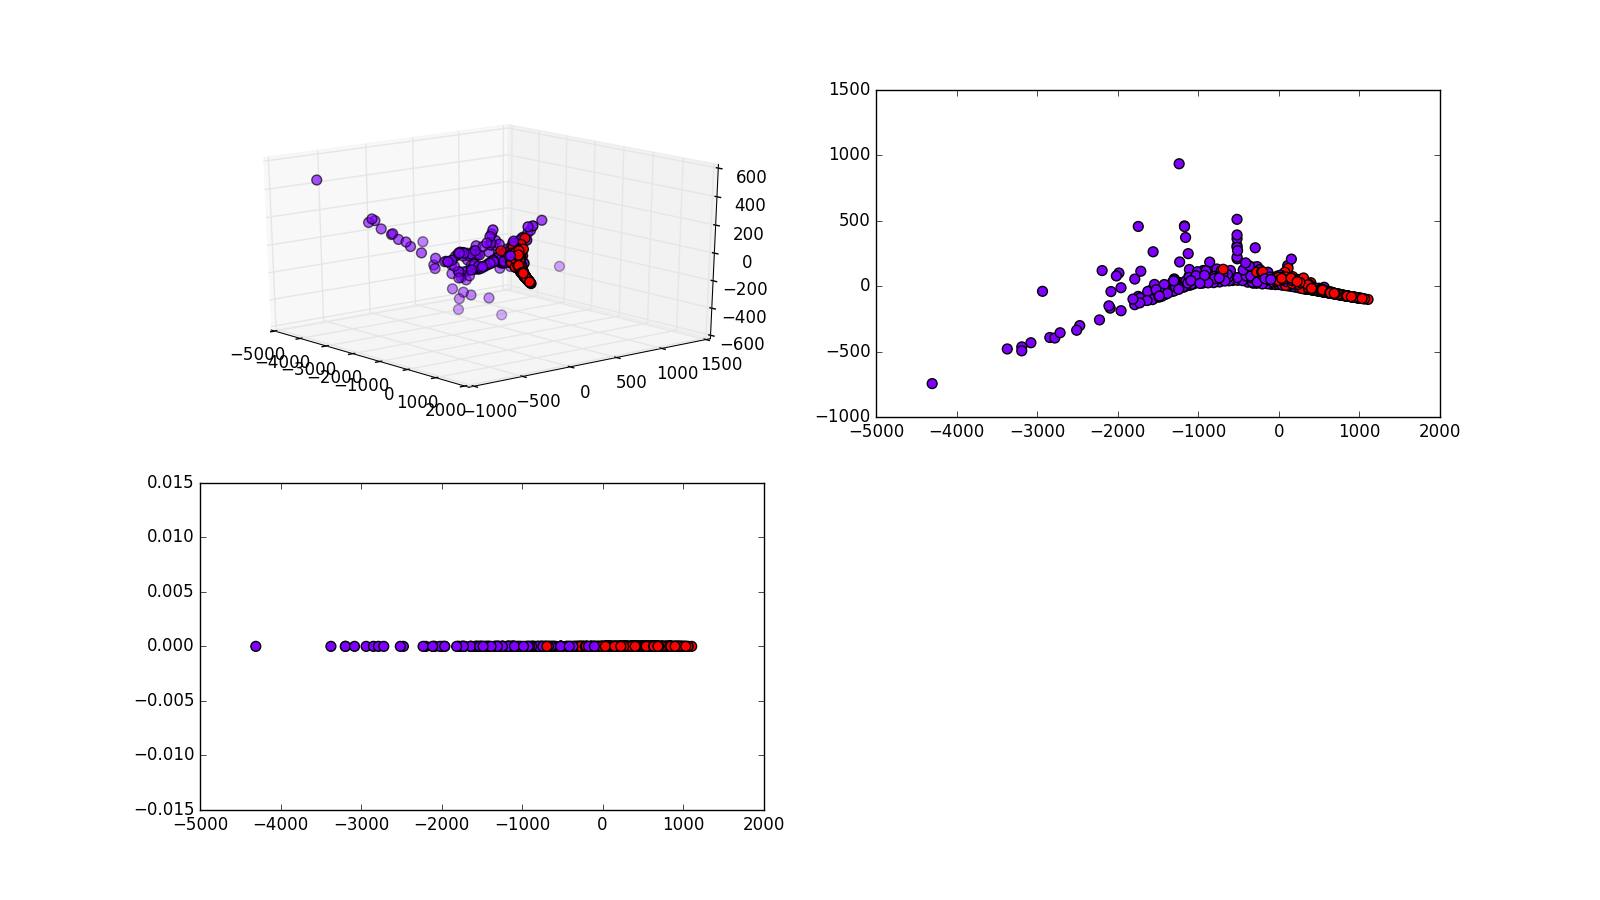
\includegraphics[width=\linewidth]{experiments/iso_wdbc}
	\caption{The reductions of WDBC to 3, 2 and 1 dimensions, respectively, with the ISOMAP algorithm.}
	\label{fig:dswdbciso}
\end{figure}

Here, prediction accuracy consistently increased when the data set was reduced.

\newpage
\subsection{Diabetes Data Set}

With 9 features observed from 768 samples collected from residents of Arizona, USA, the Diabetes data set seeks to diagnose whether a patient (sample) shows signs of diabetes (class 1) according to World Health Organization criteria or not (class 0). Is is also important to mention that only 268 samples belong, in fact, to class 1.

\begin{figure}[H]
	\centering
	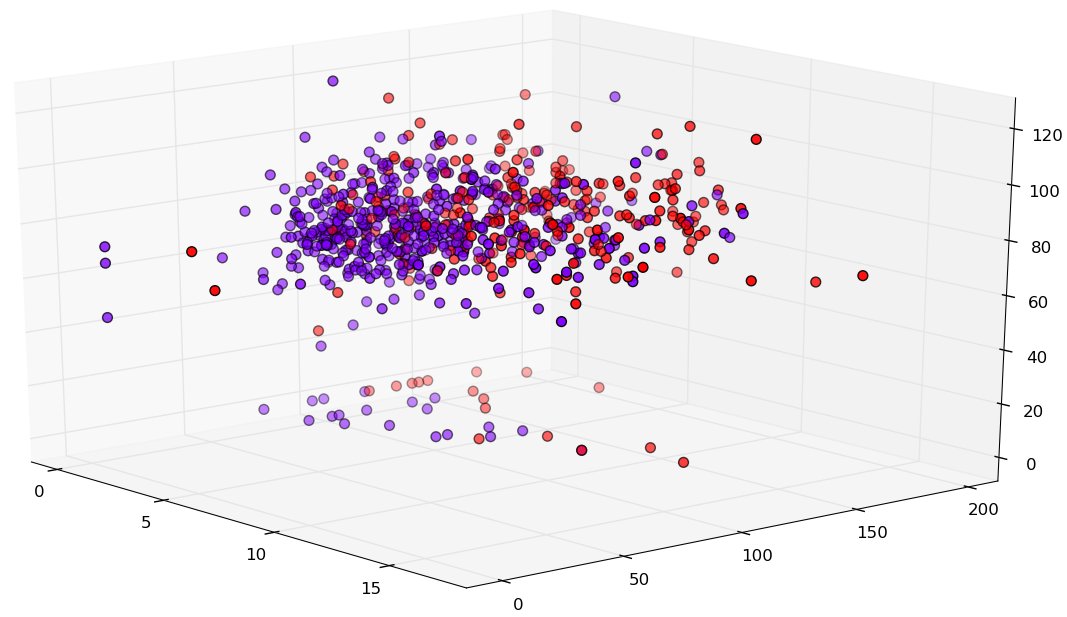
\includegraphics[width=\linewidth]{img/datasets/diabetes}
	\captionsetup{justification=centering}
	\caption{The Diabetes data set.}
	\label{fig:dsdiabetes}
\end{figure}

\newpage
\paragraph{Reducing the Diabetes Data Set With the ISOMAP Algorithm}

\begin{figure}[H]
	\centering
	\captionsetup{justification=centering}
	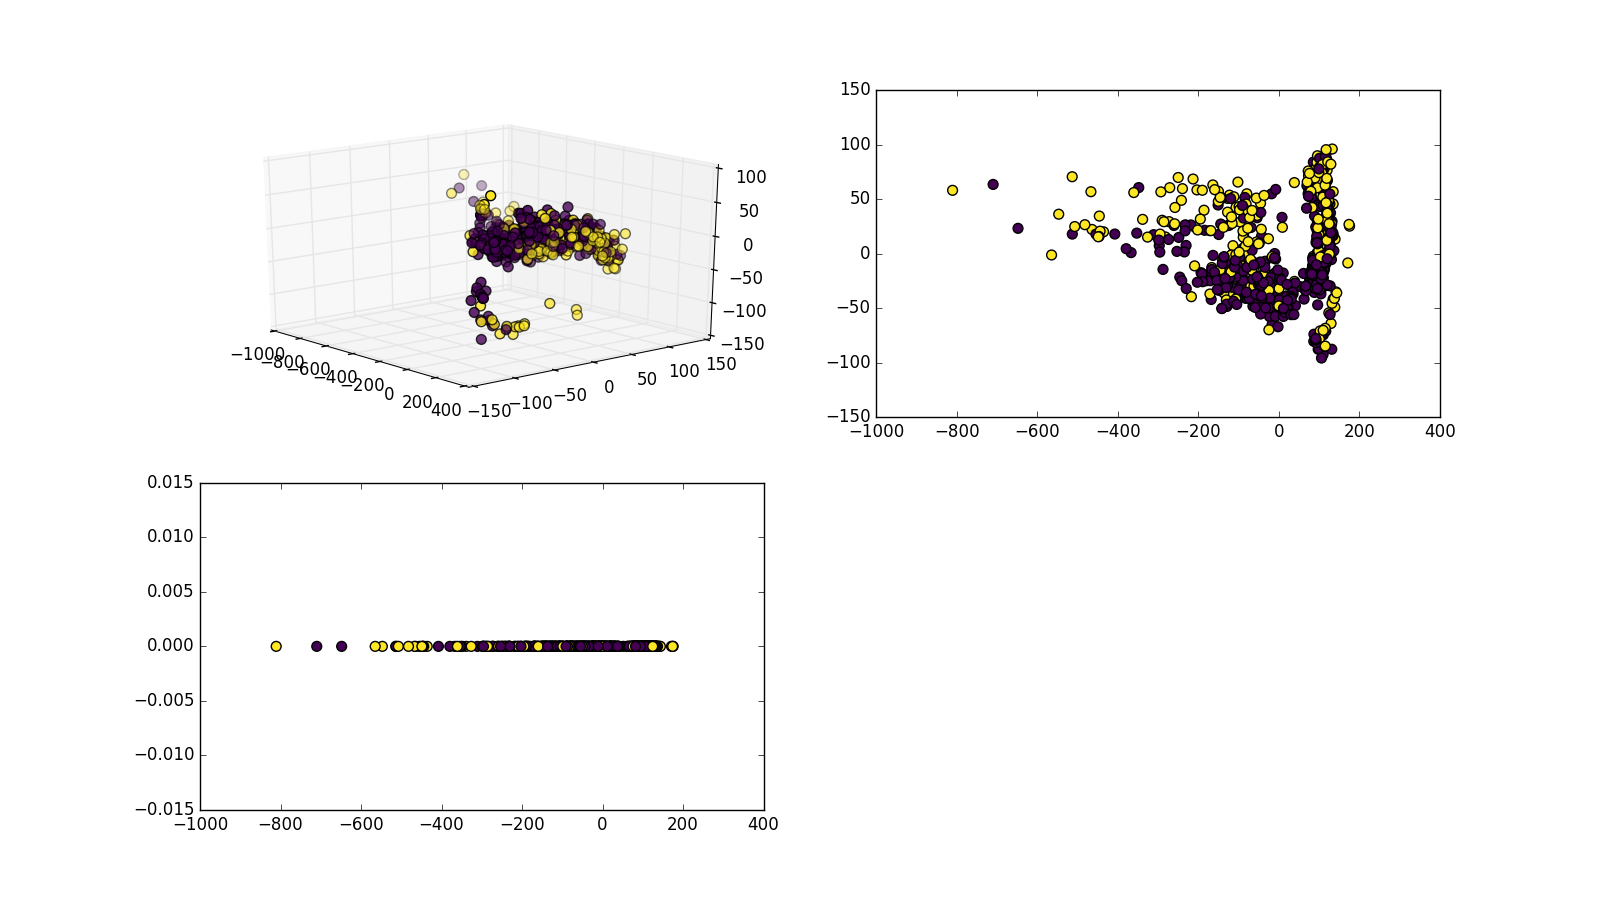
\includegraphics[width=\linewidth]{experiments/iso_diabetes}
	\caption{The reductions of Diabetes to 3, 2 and 1 dimensions, respectively, with the ISOMAP algorithm.}
	\label{fig:dsdiabetesiso}
\end{figure}

In this experiment, Diabetes was compressed to one forth of its original size (48 KB to 12 KB), and no significant prediction accuracy was lost.
